\documentclass[11pt,letterpaper]{article}
\usepackage[lmargin=1in,rmargin=1in,tmargin=1in,bmargin=1in]{geometry}
\usepackage{../style/homework}
\usepackage{../style/commands}
\setbool{quotetype}{true} % True: Side; False: Under
\setbool{hideans}{false} % Student: True; Instructor: False

% -------------------
% Content
% -------------------
\begin{document}

\homework{5: Due 03/07}{Does it disturb anyone else that `the Los Angeles Angels' baseball team translates directly to `the the angels angels'?}{Neil DeGrasse Tyson}

% Problem 1
\problem{10} Consider the region given by the following inequalities:
	\[
	\left\{
	\begin{aligned}
	x + 2y&\leq 16 \\
	-3x + y&\geq -6 \\
	x, y&\geq 0
	\end{aligned} \right.
	\]
\begin{enumerate}[(a)]
\item Is the point $(4, 5)$ in the region? Explain. Is the point $(1, 3)$ in the region? Explain. 
\item As accurately as possible, sketch the region.
\item Is the region bounded or unbounded?
\item Find the `corner points' for this region. 
\end{enumerate}

\sol
\begin{enumerate}[(a)]
\item The point $(4, 5)$ and $(1, 3)$ are in the feasible region if and only if they satisfy each of the given inequalities---which we can test (observe first that $4, 1 \geq 0$ and $5, 3 \geq 0$):
	\[
	\begin{aligned}
	x + 2y&\leq 16	&\qquad	-3x + y&\geq -6	  &\qquad 	 x + 2y&\leq 16	&	-3x + y&\geq -6 \\
	4 + 2(5)&\stackrel{?}{\leq} 16	&	-3(4) + 5&\stackrel{?}{\geq} -6	  & 	 1 + 2(3)&\stackrel{?}{\leq} 16	&	-3(1) + 3&\stackrel{?}{\geq} -6 \\
	14&\leq 16	&	-7&\geq -6	  & 	 7&\leq 16	 &	0&\geq -6 \\
	\phantom{x}&\phantom{.}\text{\cmark} & \phantom{x}&\phantom{.}\text{\xmark} & \phantom{x}&\phantom{.}\text{\cmark} & \phantom{x}&\phantom{.}\text{\cmark}
	\end{aligned}
	\]
Because the point $(4, 5)$ does not satisfy the second inequality, $(4, 5)$ is not in the region. Because $(1, 3)$ satisfies each of the given inequalities, $(1, 3)$ is in the region.

\item  Solving for $y$ in the first two inequalities, we obtain $y \leq 8 - \frac{1}{2} x$ and $y \geq 3x - 6$, respectively. We shade below the line $y= 8 - \frac{1}{2}x$ and above the line $y= 3x - 6$. Because $x, y \geq 0$, we only need examine the region in Quadrant~I. The line $y= 8 - \frac{1}{2}x$ has $y$-intercept $(0, 8)$ and the line $y= 3x - 6$ has $x$-intercept $(2, 0)$. The lines $y= 8 - \frac{1}{2}x$ and $y= 3x - 6$ intersect at the point $(4, 6)$. This gives us the region shown below.
	\[
	\fbox{
	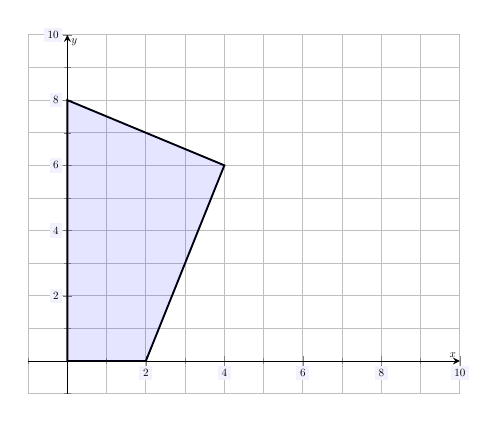
\begin{tikzpicture}[scale=0.8,every node/.style={scale=0.5}]
	\begin{axis}[
	grid=both,
	axis lines=middle,
	ticklabel style={fill=blue!5!white},
	xmin= -1, xmax=10,
	ymin= -1, ymax=10,
	xtick={0,2,4,6,8,10},
	ytick={0,2,4,6,8,10},
	minor tick = {-1,0,1,...,10},
	xlabel=\(x\),ylabel=\(y\),
	]
	\draw[line width=0.03cm] (0,0) -- (0,8) -- (4,6) -- (2,0) -- (0,0);
	\draw[line width=0.01cm,fill= blue,opacity=0.1] (0,0) -- (0,8) -- (4,6) -- (2,0) -- (0,0);
	\end{axis}
	\end{tikzpicture}
	}
	\]

\item Examining the plot in (b), we can see that the region is bounded. 

\item From the work in (b), we see that the corner points are $(0, 0)$, $(0, 8)$, $(4, 6)$, and $(2, 0)$. 
\end{enumerate}



\newpage



% Problem 2
\problem{10} Find a system of inequalities that give the following region:
	\[
	\fbox{
	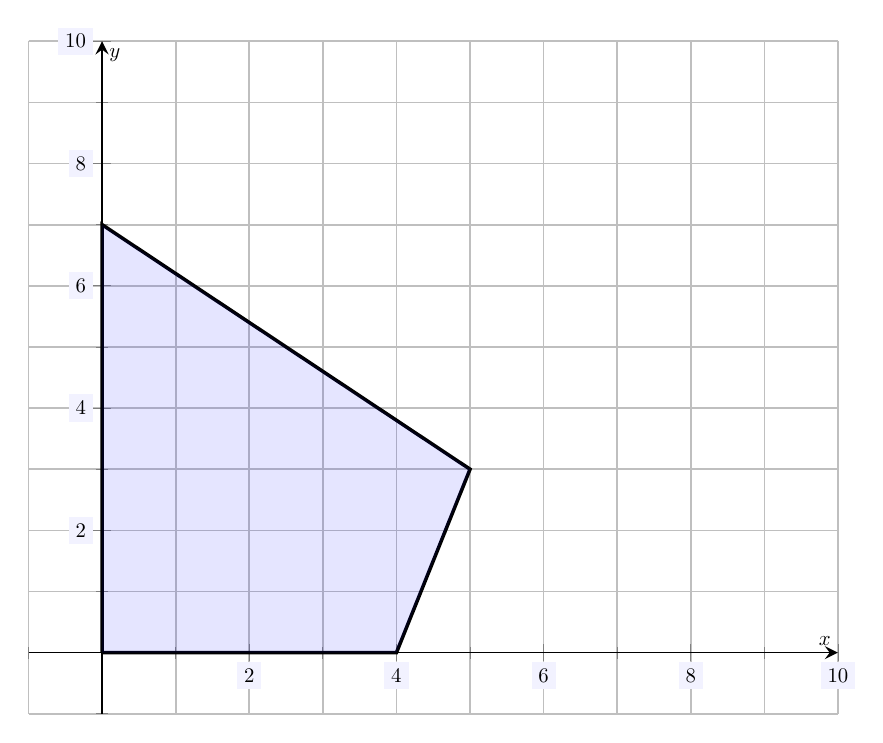
\begin{tikzpicture}[scale=1.5,every node/.style={scale=0.5}]
	\begin{axis}[
	grid=both,
	axis lines=middle,
	ticklabel style={fill=blue!5!white},
	xmin= -1, xmax=10,
	ymin= -1, ymax=10,
	xtick={0,2,4,6,8,10},
	ytick={0,2,4,6,8,10},
	minor tick = {-1,0,1,...,10},
	xlabel=\(x\),ylabel=\(y\),
	]
	\draw[line width=0.03cm] (0,0) -- (0,7) -- (5,3) -- (4,0) -- (0,0);
	\draw[line width=0.01cm,fill= blue,opacity=0.1] (0,0) -- (0,7) -- (5,3) -- (4,0) -- (0,0);
	\end{axis}
	\end{tikzpicture}
	}
	\] \pspace

\sol We have corner points $(0, 0)$, $(0, 7)$, $(5, 3)$, and $(4, 0)$. The line through $(0, 0)$ and $(0, 7)$ is clearly the line $x= 0$. We shade to the right of this line so that we have the inequality $x \geq 0$. The line through $(0, 0)$ and $(4, 0)$ is clearly the line $y= 0$. We shade above this line so we have the inequality $y \geq 0$. 

Now another inequality is given by the line through the points $(4, 0)$ and $(5, 3)$. Because this line is not vertical, we know that this line has the form $y= mx + b$. We find $m$ and $b$:
	\[
	m= \dfrac{\Delta y}{\Delta x}= \dfrac{3 - 0}{5 - 4}= \dfrac{3}{1}= 3
	\]
	\[
	y= mx + b \Longrightarrow y= 3x + b \Longrightarrow 0= 3(4) + b \Longrightarrow b= -12
	\]
Therefore, we have the line $y= 3x - 12$. Because we shade above the line, we have the inequality $y \geq 3x - 12$. Finally, the last inequality is given by the line through the points $(0, 7)$ and $(5, 3)$. Because this line is not vertical, we know that this line has the form $y= mx + b$. We find $m$ and $b$:
	\[
	m= \dfrac{\Delta y}{\Delta x}= \dfrac{3 - 7}{5 - 0}= \dfrac{-4}{5}= -\dfrac{4}{5}
	\]
	\[
	y= mx + b \Longrightarrow y= -\frac{4}{5}\,x + b \Longrightarrow 7= -\frac{4}{5} \cdot 0 + b \Longrightarrow b= 7
	\]
Therefore, we have the line $y= -\frac{4}{5}\,x + 7$. Because we shade below the line, we have the inequality $y \leq -\frac{4}{5}\,x + 7$. Therefore, the inequalities that determine this region are\dots
	\[
	\begin{cases}
	y \geq 3x - 12 \\
	y \leq -\frac{4}{5}\,x + 7 \\
	x, y \geq 0
	\end{cases}
	\]



\newpage



% Problem 3
\problem{10} Use the Fundamental of Theorem of Linear Programming to find the maximum and minimum values for the function $f(x, y)$ below given the constraints---also given below.
	\[
	f(x,y)= x + 3y 
	\]
	\[
	\left\{
	\begin{aligned}
	x + 5y&\leq 25 \\
	x + y&\leq 9 \\
	-2x + y&\geq -12 \\
	x, y&\geq 0
	\end{aligned} \right.
	\] \pspace

\sol First, we sketch the region given by these inequalities. Solving for $y$ in the first three inequalities, we obtain $y \leq -\frac{1}{5}\,x + 5$, $y \leq -x + 9$, and $y \geq 2x - 12$, respectively. Sketching this region carefully, we obtain the plot below.
	\[
	\fbox{
	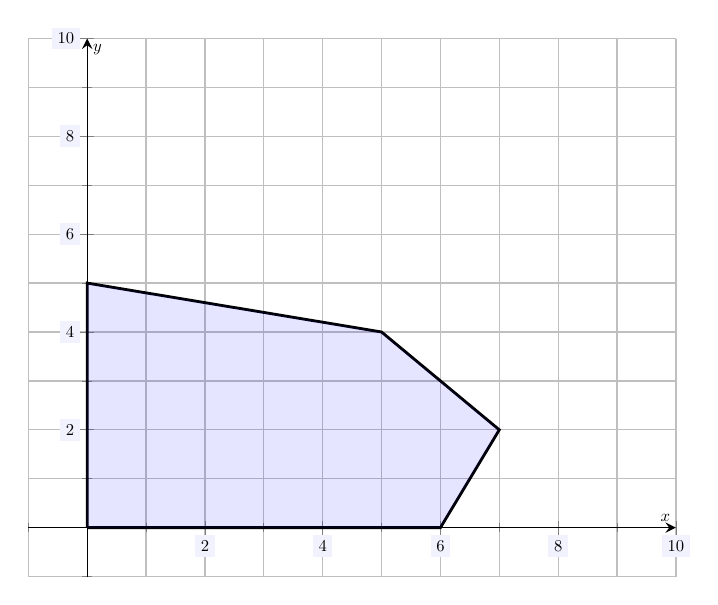
\begin{tikzpicture}[scale=1.2,every node/.style={scale=0.5}]
	\begin{axis}[
	grid=both,
	axis lines=middle,
	ticklabel style={fill=blue!5!white},
	xmin= -1, xmax=10,
	ymin= -1, ymax=10,
	xtick={0,2,4,6,8,10},
	ytick={0,2,4,6,8,10},
	minor tick = {-1,0,1,...,10},
	xlabel=\(x\),ylabel=\(y\),
	]
	\draw[line width=0.03cm] (0,0) -- (0,5) -- (5,4) -- (7,2) -- (6,0) -- (0,0);
	\draw[line width=0.01cm,fill= blue,opacity=0.1] (0,0) -- (0,5) -- (5,4) -- (7,2) -- (6,0) -- (0,0);
	\end{axis}
	\end{tikzpicture}
	}
	\] 
Because this region is nonempty and bounded, the Fundamental Theorem of Linear Programming applies. Therefore, the function $f(x, y)$ has a maximum and minimum value on this region and they must occur at a corner point for the region. We find the corner points. \pspace

Clearly, $(0, 0)$ is a corner point. The `upper left' corner point is the $y$-intercept of the line $y= -\frac{1}{5}\,x + 5$, which is $(0, 5)$. The `upper middle' corner point is the intersection of the lines $y= -\frac{1}{5}\,x + 5$ and $y= -x + 9$, which is $(5, 4)$. The `rightmost' corner point is the intersection of the lines $y= -x + 9$ and $y= 2x - 12$, which is $(7, 2)$. Finally, the `bottom right' corner point is the $x$-intercept of the line $y= 2x - 12$, which is $(6, 0)$. Now we test the function at each corner point:
	\begin{table}[!ht]
	\centering
	\begin{tabular}{l | l}
	Corner Point & $f(x, y)$ \\ \hline
	$(0, 0)$ & $f(0, 0)= 0 + 3(0)= 0$ \\
	$(0, 5)$ & $f(0, 5)= 0 + 3(5)= 15$ \\
	$(5, 4)$ & $f(5, 4)= 5 + 3(4)= 17$ \\
	$(7, 2)$ & $f(7, 2)= 7 + 3(2)= 13$ \\
	$(6, 0)$ & $f(6, 0)= 6 + 3(0)= 6$
	\end{tabular}
	\end{table} \par
Therefore, the minimum is $0$ and occurs at $(0, 0)$ and the maximum is $17$ and occurs at $(5, 4)$. 



\newpage



% Problem 4
\problem{10} Consider the maximization problem given below:
	\[
	\text{max } z= x_1 + 3x_2 - 2x_3
	\]
	\[
	\left\{
	\begin{aligned}
	x_1 + x_2 + x_3&\leq 8 \\
	2x_1 - 3x_2 + x_3&\leq 5 \\
	-x_1 + 4x_2 - 2x_3&\leq 2 \\
	x_1, x_2, x_3&\geq 0
	\end{aligned} \right.
	\]
\begin{enumerate}[(a)]
\item Does the point $(-1, 0, 1)$ satisfy the inequalities above? Explain.
\item Is the point $(2, 3, 1)$ in the feasible region? Explain. 
\item Is the point $(2, 1, 2)$ a feasible point? Explain. If this is a feasible point, find the corresponding $z$ value.
\item Can $(2, 1, 2)$ be a solution to this maximization problem? Explain. [Hint: Can you change some of the variables `a bit' to increase $z$ while still satisfying all the inequalities?]
\end{enumerate} 

\sol
\begin{enumerate}[(a)]
\item The point $(x_1, x_2, x_3)= (-1, 0, 1)$ clearly does not satisfy the inequalities above because $x_1= -1 \not\geq 0$. 

\item The point $(x_1, x_2, x_3)= (2, 3, 1)$ is a feasible point if it satisfies all the inequalities above. We can simply test this (note that $2, 3, 1 \geq 0$): 
	\[
	\begin{aligned}
	x_1 + x_2 + x_3&\leq 8 &\qquad 2x_1 - 3x_2 + x_3&\leq 5 &\qquad -x_1 + 4x_2 - 2x_3&\leq 2 \\
	2 + 3 + 1&\stackrel{?}{\leq} 8 & 2(2) - 3(3) + 1&\stackrel{?}{\leq} 5 & -2 + 4(3) - 2(1)&\stackrel{?}{\leq} 2 \\
	6&\leq 8 & -4&\leq 5 & 8&\leq 2 \\
	\phantom{x}&\phantom{x}\text{\cmark} & \phantom{x}&\phantom{x}\text{\cmark} & \phantom{x}&\phantom{x}\text{\xmark}
	\end{aligned}
	\]
Because $(2, 3, 1)$ does not satisfy all the above inequalities, $(2, 3, 1)$ is not a feasible point. 

\item The point $(x_1, x_2, x_3)= (2, 1, 2)$ is a feasible point if it satisfies all the inequalities above. We can simply test this (note that $2, 1 \geq 0$): 
	\[
	\begin{aligned}
	x_1 + x_2 + x_3&\leq 8 &\qquad 2x_1 - 3x_2 + x_3&\leq 5 &\qquad -x_1 + 4x_2 - 2x_3&\leq 2 \\
	2 + 1 + 2&\stackrel{?}{\leq} 8 & 2(2) - 3(1) + 2&\stackrel{?}{\leq} 5 & -2 + 4(1) - 2(2)&\stackrel{?}{\leq} 2 \\
	5&\leq 8 & 3&\leq 5 & -2&\leq 2 \\
	\phantom{x}&\phantom{x}\text{\cmark} & \phantom{x}&\phantom{x}\text{\cmark} & \phantom{x}&\phantom{x}\text{\cmark}
	\end{aligned}
	\]
Because $(2, 3, 1)$ does satisfies all the above inequalities, $(2, 1, 2)$ is a feasible point. The $z$ value at this feasible point is $z(2, 1, 2)= 2 + 3(1) - 2(2)= 1$. 
 
\item The function $z= x_1 + 3x_2 - 2x_3$ is increasing in $x_1, x_2$ and decreasing in $x_3$. Therefore, if we can decrease $x_3$ from $2$ to $0$, i.e. move from the point $(2, 1, 2)$ to the point $(2, 1, 0)$, we can increase $z$ while staying in the feasible region. It is routine to verify that $(2, 1, 0)$ satisfies all the above inequalities, i.e. is a feasible point. Because $z$ has value $1$ at $(2, 1, 2)$ and value $5$ at $(2, 1, 0)$, we know that $(2, 1, 2)$ cannot be a location of a maximum for $z$ on this region. 
\end{enumerate}



\newpage



% Problem 5
\problem{10} Write the initial simplex tableau corresponding to the standard maximization problem given below: 
	\[
	\text{max } z= 3x_1 - 4x_2 + x_3
	\]
	\[
	\left\{
	\begin{aligned}
	2x_1 - x_2 &+ 4x_3\leq 8 \\
	x_1 + 6x_3&\leq 5 \\
	x_1, x_2, x_3&\geq 0
	\end{aligned} \right.
	\] \pspace

\sol First, we move every variable in $z= 3x_1 - 4x_2 + x_3$ to the `$z$'-side of the equation to obtain $z - 3x_1 + 4x_2 - x_3= 0$. Now we add slack variables to the appropriate inequalities to turn them to equalities and add the `$z$-equation below these, being careful to align all the decision variables: \pspace
	\begin{table}[!ht]
	\centering
	\begin{tabular}{ccccccccccc}
		&	 & $2x_1$ & $-$ & $x_2$ & $+$ & $4x_3$ & $+$ & $s_1$ & & $= 8$ \\	
		&	 & $x_1$ & $+$ & $0x_2$ & $+$ & $6x_3$ & $+$ & & $s_2$ & $= 5$ \\	
	$z$   & $-$ & $3x_1$ & $+$ & $4x_2$ & $-$ & $x_3$ & $+$ & & & $= 0$ 
	\end{tabular}
	\end{table} \pspace
This gives us an initial simplex tableau of\dots \pspace
	 \begin{table}[!ht]
	\centering
	\begin{tabular}{rrrrr|r}
	$2$ & $-1$ & $4$ & $1$ & $0$ & $8$ \\
	$1$ & $0$ & $6$ & $0$ & $1$ & $5$ \\ \hline
	$-3$ & $4$ & $-1$ & $0$ & $0$ & $0$ \\
	\end{tabular}
	\end{table}



\newpage



% Problem 6
\problem{10} Below is the final simplex tableau corresponding to a standard maximization problem:
	\begin{table}[!ht]
	\centering
	\begin{tabular}{rrrrrrr|r}
	$0$ & $-0.286$ & $0$ & $-0.929$ & $1$ & $-0.071$ & $-0.357$ & $321.0$ \\
	$1$ & $1.07$ & $0$ & $1.36$ & $0$ & $0.143$ & $0.214$ & $607.0$ \\
	$0$ & $0.214$ & $1$ & $0.571$ & $0$ & $-0.071$ & $0.143$ & $71.4$ \\ \hline
	$0$ & $31.8$ & $0$ & $44.3$ & $0$ & $6.38$ & $15.3$ & $35771.43$
	\end{tabular}
	\end{table} 
\begin{enumerate}[(a)]
\item How many inequalities were there for this problem?
\item How many slack variables are present for this problem?
\item How many decision variables were there for this problem?
\item Write the solution to this maximization problem. Your solution should include the maximum values as well as the values for all the decision and slack variables.
\end{enumerate} \pspace

\sol
\begin{enumerate}[(a)]
\item The last row of the simplex tableau corresponds to the `function equation.' The other rows correspond to the inequalities in the initial problem. Therefore, there were initially three inequalities. 
 
\item For each inequality, we introduced a slack variable. By (a), we know that there were three inequalities in the original problem. Therefore, there were three slack variables. 

\item The last column corresponds to the `solution vector.' The remaining columns either correspond to a decision variable or a slack variable. By (b), we know that there were three slack variables. Because there are seven columns, this means that there are four decision variables. 

\item The basic variables are clearly the variables corresponding to columns one, three, and five, which correspond to variables $x_1$, $x_3$, and $s_1$, respectively. Reading off their corresponding values in the solution vector, we see that $x_1= 607.0$, $x_3= 71.4$, and $s_1= 321.0$. The other variables are nonbasic variables; hence, all the remaining variables are zero. Therefore, we have solution $(x_1, x_2, x_3, x_4, s_1, s_2, s_3)= (607.0, 0, 71.4, 0, 321.0, 0, 0)$. At this point, the corresponding function value (read in the bottom rightmost entry) is $35771.43$.
\end{enumerate}


\end{document}